\documentclass{beamer}

\usepackage{amsmath}
\usepackage{booktabs}
\usepackage{tabularx}
\usepackage{rotating}
\usepackage{microtype}
\usepackage{indentfirst}
\usepackage{amssymb}
\usepackage{graphicx}
\usepackage{tikz}
\usetikzlibrary{arrows}
\usepackage{lmodern}
\usepackage[T1]{fontenc}
\usepackage[utf8x]{inputenc}

\usetheme[secheader]{Boadilla}
\usecolortheme{beaver}

% Defining some color scheme
\setbeamercolor*{item}{fg=red}
\defbeamertemplate*{itemize subitem}{default}{\tiny\raise1.5pt\hbox{\donotcoloroutermaths$\blacktriangleright$}}
\setbeamercolor*{block title}{fg=black!30!red,bg=black!20}
\setbeamercolor*{block body}{fg=black,bg=black!10}

\title[SecureIt]{SecureIt}
\author{Luca Bonato, Marco Ziccardi}
\date{Wireless Network}
\institute[UniPD]{University of Padua\\\includegraphics[width=15mm]{./../ipermediali/img/unipd_logo.pdf}}


\begin{document}

\begin{frame}
\begin{minipage}[l]{.7\textwidth}
~\\[4cm]\includegraphics[width=3.5cm]{./../ipermediali/img/icona.pdf}
\end{minipage}\begin{minipage}[r]{.5\textwidth}
~\\[4cm]\includegraphics[width=3.5cm]{./../ipermediali/img/icona.pdf}
\end{minipage}\\[-6.5cm]
\maketitle
\end{frame}

\begin{frame}
\frametitle{Table of contents}
\tableofcontents
\end{frame}

% INTRODUCTION
\section{Introduction}
\begin{frame}
\frametitle{Application overview}
\begin{block}{SecureIt}
An application to turn an Android device into a home-security and device-tracking system. It tries to exploit all the device functions to offer a wide range of security mechanisms.
\end{block}
Other applications in the market try to offer security using only a fraction of devices' abilities
\begin{itemize}
	\item \textbf{Motion Detector Pro}: only motion detection
	\item \textbf{Sound Detector}: only noise detection
	\item \textbf{Surveillance}: motion and sound detection but not shake detection and device tracking
\end{itemize}
\end{frame}

\begin{frame}
\frametitle{Architecture}
\begin{center}
\includegraphics[scale=.4]{./../../relazioni/wireless/resources/architecture.pdf}
\end{center}
\end{frame}

\section{Detection mechanisms}
\begin{frame}
\frametitle{Shake detection}
\begin{block}{}
The \textbf{accelerometer} is used to detect motion of the phone itself. The accelerations on the 3 axis computed by the accelerometer are used to estimate the intensity of phone's shake. The alert is fired only if this intensity is over the threshold specified by the user.
\end{block}
\begin{minipage}[c]{.7\textwidth}
{\footnotesize\[\frac{(\Delta accel_X) + (\Delta accel_Y) + (\Delta accel_Z)}{\Delta t} > \texttt{THRESHOLD}\]}
\end{minipage}\begin{minipage}[c]{.25\textwidth}
\includegraphics[scale=.3]{./../ipermediali/img/accelerometer.png}
\end{minipage}
\end{frame}

\begin{frame}
\frametitle{Motion detection}
\begin{block}{}
The \textbf{camera} is used to detect motion in the surrounding environment. The frames capured by the camera are compared to determine variations between them: if the differences of two consecutive frames are over the threshold specified by the user an alert is fired. The application tries also to upload the captured frames so that the user can check what happened.
\end{block}
\begin{minipage}[c]{.25\textwidth}
\includegraphics[scale=.15]{./../ipermediali/img/camera.png}
\end{minipage}\begin{minipage}[c]{.65\textwidth}
\begin{itemize}
  \item Using a simple motion detection algorithm
  \item Threshold specifies when two pixels are different and the amount of different pixels needed to detect motion
  \item Stores the captured frames in case an alarm is fired
\end{itemize}
\end{minipage}
\end{frame}

\begin{frame}
\frametitle{Noise detection}
\begin{block}{}
The \textbf{microphone} is used to detect an abnormal noise level in the surrounding environment. The sound sampled by the microphone is converted to a decibel scale. When the sampled and converted values exceed the threshold set by the user an alert is fired and the application records 10 seconds of environment noise. The application tries also to upload the recorded audio to let the user hear what happened.
\end{block}
\begin{minipage}[c]{.25\textwidth}
\includegraphics[scale=.15]{./../ipermediali/img/microphone.png}
\end{minipage}\begin{minipage}[c]{.65\textwidth}
\begin{itemize}
  \item An average of sampled noise is considered and then converted
    {\footnotesize\[dB_i = 10\log_{10} \left(\frac{V_i}{V_o}\right)^2\]}
  \item 3 possible threshold level displayed in UI
  \item Records audio only when needed
\end{itemize}
\end{minipage}
\end{frame}


\section{Upload info}
\begin{frame}
\frametitle{Alert communication}
\begin{block}{}
Based on selected preferences the application tries to alert the user of an abnormal status of the environment or of the device: no use of a securety system if it can't alert someone of an intrusion.
\end{block}
\begin{itemize}
  \item SMS: just sends a message to the user to notify an abnormal status
  \item Upload info to back-end: sends captured images and audio to the specified server
  \item Collaborative help: seeks help from other devices to upload some information to the specified server
\end{itemize}
\end{frame}

\begin{frame}
\frametitle{Back-end}
\begin{block}{}
Having the device storing the information related to the intrusion is not wise: the device itself can be stolen. It's necessary to store the information to a safe place: a dedicated \textbf{remote server}.\\This way the user can access the information anywhere and anytime: no need to have the device (that could be already stolen).
\end{block}
The information to upload can be too resource-consuming:
\begin{itemize}
  \item WiFi connection: no bandwidth constraint. The application tries to upload every gathered information (every captured image, recorded audio, device location)
  \item 3G connection: bandwidth constraint. The application tries to upload a subset of the gathered information (half of the captured images, recorder audio, device location)
\end{itemize}
\end{frame}

\begin{frame}
\frametitle{Back-end communication}
The server offers REST API. Through these API it's possibile to upload data to the server.\\
To organize the data, the server has to know to whom the data are related: the user must be registered to be able to use the server storage mechanism. The user can therefore login to browse all the data gathered from his devices.\\
The server accepts 3 kind of information:
\begin{enumerate}
  \item Images: \texttt{\lbrack POST\rbrack	/api/phones/:phoneId/images}
  \item Audio: \texttt{\lbrack POST\rbrack 	/api/phones/:phoneId/audio}
  \item Location: \texttt{\lbrack POST\rbrack  /api/phones/:phoneId/positions}\\
                  ~~~~~\texttt{\lbrack POST\rbrack  /api/phones/:phoneId/position/delegated}
\end{enumerate}
\end{frame}

\begin{frame}
\frametitle{Back-end access}
\begin{block}{}
Information upload is a sensible operation: the server must be sure that the information is real and not uploaded to mislead the user. Only data sent by authorized devices can be stored in the server.
\end{block}
At login the application retrieves the credentials needed to upload data:\\
\texttt{[POST] /user/accesstoken}\\
The credentials are sent to the application in JSON:
\begin{itemize}
  \item \texttt{access\_token}: used to authenticate the device to the server
  \item \texttt{delegated\_access\_token}: used to authenticate the information sent to the server by another device
\end{itemize}
\end{frame}

\begin{frame}
\frametitle{Upload images and audio}
Images and audio are uploaded to the back-end in a similar way.\\
A \texttt{MULTIPART POST} request is sent to the appropriate REST API.\\
Images and audio are uploaded only by the user device: \texttt{access\_token} is inserted in the request header for the authentication.
\begin{center}
\includegraphics[scale=.22]{./../ipermediali/img/slideshow.png}
\end{center}
\end{frame}

\begin{frame}
\frametitle{Device location}
If some connection is available (WiFi or 3G) the application sends periodically to the server information about the location of the device (to track it down if it is stolen). The location is expressed by geographic coordinates taken by GPS (if active) or by some geolocalization service.
\begin{center}
\includegraphics[scale=.22]{./../ipermediali/img/map.png}
\end{center}
\end{frame}

\section{Bluetooth}
\begin{frame}
\frametitle{Delegated upload}
\begin{block}{}
If no connection is available the application activates a collaborative protocol based on opportunistic bluetooth connections.\\
The application delegates another device to upload its location, so that at least device-tracking is possible.
\end{block}
The application seeks helps from other devices: it asks to upload some info to the server.
\begin{itemize}
  \item Data sent to the server must be authorized: a little authentication protocol is implemented
  \item Bluetooth connection should not request user approval: untrusted bluetooth connection is used, so no explicit confirmation by the user is needed
\end{itemize}
Bluetooth connections cannot withstand heavy traffic:
\begin{itemize}
  \item no request for images or audio upload are made
  \item just a request to upload the location of the device
\end{itemize}
\end{frame}

\begin{frame}
\frametitle{Collaborative help workflow}
\begin{enumerate}
  \item Bluetooth discovery is started
  \item Tries to create a bluetooth connection with each discovered device
  \item If the connection is not discardet a digital sign protocol is started
  \includegraphics[scale=.2]{./../ipermediali/img/bluetooth.png}
  \item If location is sent correctly 1 hour is waited before next retransmission, otherwise only 1 minute is waited
\end{enumerate}
\end{frame}

\begin{frame}
\frametitle{Signing protocol}
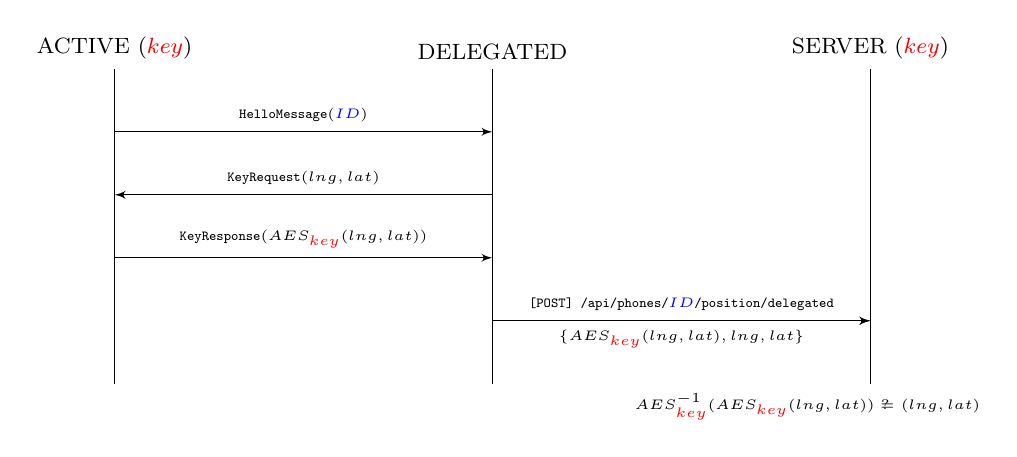
\begin{tikzpicture}[scale=.8]
\draw (0,0) node[above]{\footnotesize ACTIVE ({$\color{red}key$})} -- (0, -5);
\draw (6,0) node[above]{\footnotesize DELEGATED} -- (6, -5);
\draw (12,0) node[above]{\footnotesize SERVER ({$\color{red}key$})} -- (12, -5);

\draw[->,>=latex'] (0,-1) -- (6,-1)node[above,midway]{\tiny \texttt{HelloMessage}({$\color{blue}ID$})};
\draw[<-,>=latex'] (0,-2) -- (6,-2)node[above,midway]{\tiny \texttt{KeyRequest}($lng,lat$)};
\draw[->,>=latex'] (0,-3) -- (6,-3)node[above,midway]{\tiny \texttt{KeyResponse}($AES_{\color{red}key}(lng,lat)$)};
\draw[->,>=latex'] (6,-4) -- (12,-4)node[above,midway]{\tiny \texttt{[POST] /api/phones/{$\color{blue}ID$}/position/delegated}};
\draw[->,>=latex'] (6,-4) -- (12,-4)node[anchor=north,midway]{\tiny\{$AES_{\color{red}key}(lng,lat), lng,lat$\}};
\draw (11,-5)node[anchor=north]{\tiny $AES^{-1}_{\color{red}key}(AES_{\color{red}key}(lng,lat)) =\!\!\!\!?\;\; (lng,lat)$};
\end{tikzpicture}
\end{frame}

\end{document}
